\newcommand{\docshort}{Fundamentos e arquitetura}
% preâmbulo comum — ambiente sem lmodern: ae + aecompl (regras do projeto)
\documentclass[11pt,a4paper]{article}
\usepackage{ae,aecompl}
\usepackage[utf8]{inputenc}
\IfFileExists{brazil.ldf}{\usepackage[brazil]{babel}}{}
\usepackage[a4paper,margin=2.3cm]{geometry}
\usepackage{amsmath,amssymb,amsthm,mathtools}
\usepackage{booktabs,array,longtable}
\usepackage{enumitem}
\usepackage{xcolor}
\usepackage{graphicx}
\usepackage{tikz}
\usetikzlibrary{arrows.meta,positioning,fit,calc}
\usepackage[most]{tcolorbox}
\usepackage{listings}
\usepackage[ruled,vlined,linesnumbered]{algorithm2e}
\usepackage{microtype}
\usepackage{fancyhdr}
\usepackage{float}
\usepackage[colorlinks=true,linkcolor=blue!60!black,citecolor=blue!60!black,urlcolor=blue!60!black]{hyperref}
\setlength{\emergencystretch}{1.5em}
% marcadores em modo matemático (TS1 sem face vetorial sob ae)
\renewcommand{\labelitemi}{$\bullet$}
\renewcommand{\labelitemii}{$\circ$}
\renewcommand{\labelitemiii}{$\ast$}
% nomes em português sem depender do babel
\renewcommand{\contentsname}{Sumário}
\renewcommand{\refname}{Referências}
\renewcommand{\figurename}{Figura}
\renewcommand{\tablename}{Tabela}
\renewcommand{\abstractname}{Resumo}
\renewcommand{\proofname}{Demonstração}
\SetAlgorithmName{Algoritmo}{Algoritmo}{Lista de Algoritmos}
\definecolor{tune3blue}{RGB}{31,73,125}
\definecolor{okgreen}{RGB}{20,110,60}
\definecolor{warnred}{RGB}{160,30,30}
\definecolor{codebg}{RGB}{245,246,248}
\lstset{basicstyle=\ttfamily\small,backgroundcolor=\color{codebg},frame=single,rulecolor=\color{gray!40},
  breaklines=true,columns=fullflexible,keepspaces=true,showstringspaces=false,
  language=Python,keywordstyle=\color{tune3blue}\bfseries,commentstyle=\color{gray!70!black}\itshape,
  literate={á}{{\'a}}1 {à}{{\`a}}1 {ã}{{\~a}}1 {â}{{\^a}}1 {é}{{\'e}}1 {ê}{{\^e}}1 {í}{{\'i}}1 {ó}{{\'o}}1 {ô}{{\^o}}1 {õ}{{\~o}}1 {ú}{{\'u}}1 {ç}{{\c{c}}}1 {Á}{{\'A}}1 {É}{{\'E}}1 {Í}{{\'I}}1 {Ó}{{\'O}}1 {Ú}{{\'U}}1 {Ç}{{\c{C}}}1 {Ã}{{\~A}}1 {Õ}{{\~O}}1 {Ê}{{\^E}}1 {Ô}{{\^O}}1 {Â}{{\^A}}1 {²}{{$^2$}}1 {·}{{$\cdot$}}1 {≥}{{$\geq$}}1 {≤}{{$\leq$}}1 {→}{{$\to$}}1 {∈}{{$\in$}}1 {∞}{{$\infty$}}1 {σ}{{$\sigma$}}1 {ρ}{{$\rho$}}1 {γ}{{$\gamma$}}1 {η}{{$\eta$}}1 {θ}{{$\theta$}}1 {Σ}{{$\Sigma$}}1 {λ}{{$\lambda$}}1 {ε}{{$\varepsilon$}}1 {–}{{--}}1 {—}{{---}}1 {×}{{$\times$}}1}
\newtcolorbox{ideia}[1][]{colback=tune3blue!5,colframe=tune3blue,fonttitle=\bfseries,title={#1},breakable}
\newtcolorbox{alerta}[1][]{colback=warnred!5,colframe=warnred,fonttitle=\bfseries,title={#1},breakable}
\newtcolorbox{codigo}[1][]{colback=okgreen!4,colframe=okgreen,fonttitle=\bfseries,title={#1},breakable}
\theoremstyle{definition}
\newtheorem{definicao}{Definição}[section]
\newtheorem{proposicao}{Proposição}[section]
\newtheorem{exemplo}{Exemplo}[section]
\newtheorem{observacao}{Observação}[section]
\DeclareMathOperator{\Tr}{Tr}
\DeclareMathOperator{\CVaR}{CVaR}
\DeclareMathOperator{\VaR}{VaR}
\DeclareMathOperator{\Var}{Var}
\DeclareMathOperator{\Cov}{Cov}
\DeclareMathOperator{\GSNR}{GSNR}
\DeclareMathOperator*{\argmin}{arg\,min}
\newcommand{\R}{\mathbb{R}}
\newcommand{\E}{\mathbb{E}}
\newcommand{\norm}[1]{\left\lVert #1 \right\rVert}
\newcommand{\code}[1]{\texttt{#1}}
\pagestyle{fancy}\fancyhf{}
\rhead{\small Tune3 — \docshort}
\lhead{\small UNIPAMPA / AI Horizon Labs}
\cfoot{\thepage}


\title{\textbf{Tune3}\\[4pt]\Large Otimização de hiperparâmetros consciente de curvatura para detecção de malware\\[6pt]
\large Um guia autocontido: do problema à implementação}
\author{Projeto Tune3 --- coordenação: Prof.\ Dionatan R.\ Schmidt\\ UNIPAMPA, Campus Alegrete --- AI Horizon Labs}
\date{Versão de 21 de setembro de 2026 (revisão 2) --- alinhada ao commit pós-auditoria do repositório \code{dionatanschmidt/tune3}}

\begin{document}
\maketitle

\begin{abstract}
Este documento explica, sem pressupor leitura prévia, o que o Tune3 faz, por que faz e como cada peça está implementada. Ele foi escrito para uma pessoa que queira \emph{entender} o projeto --- um aluno novo, um colaborador de outra área ou um revisor --- e não para vender uma tese: onde a evidência é forte, dizemos; onde ela é fraca ou inexistente, também dizemos. Toda afirmação sobre o código refere-se ao estado do repositório após a auditoria de setembro de 2026; toda afirmação sobre a literatura refere-se ao que os artigos de fato estabelecem, conforme a leitura corrigida do próprio projeto.
\end{abstract}

\tableofcontents
\newpage

% =====================================================================
\section{Como ler este documento}

O texto avança em camadas. As Seções~\ref{sec:problema} a~\ref{sec:proxy} constroem a motivação (por que \emph{risco de cauda}, por que \emph{curvatura}). As Seções~\ref{sec:hutchinson} a~\ref{sec:guardas} explicam cada componente matemático com a mesma notação que aparece no código. A Seção~\ref{sec:algoritmo} monta o algoritmo completo. A Seção~\ref{sec:evidencia} apresenta o estado da evidência e a tensão científica que a próxima rodada de experimentos precisa resolver. A Seção~\ref{sec:literatura} lista o que cada artigo do corpus sustenta --- e o que não sustenta. O Apêndice~\ref{ap:mapa} mapeia cada símbolo a um arquivo e uma classe.

\begin{ideia}[Convenção de honestidade]
Usamos três rótulos ao longo do texto. \textbf{RESULTADO}: algo demonstrado ou verificado computacionalmente. \textbf{HIPÓTESE}: algo que o projeto \emph{aposta} e ainda está testando. \textbf{DECISÃO DE PROJETO}: uma escolha de engenharia que poderia ter sido outra. Confundir os três é o erro mais comum em textos sobre este tipo de método.
\end{ideia}

% =====================================================================
\section{O problema: a média não protege ninguém}\label{sec:problema}

Um detector de malware é, do ponto de vista estatístico, um classificador $f_\theta$ com parâmetros $\theta\in\R^W$ treinado para minimizar o \emph{risco empírico}
\[
\min_\theta\; \E_{(x,y)\sim P}\big[\,L(f_\theta(x),y)\,\big],
\]
onde $L$ é uma perda (aqui, entropia cruzada ponderada por classe). Essa formulação otimiza o \emph{caso médio}. Um centro de operações de segurança (SOC), porém, não é avaliado pela média: ele é avaliado pelo pior caso --- o dia em que uma família nova de malware passa despercebida ou em que um lote de aplicativos legítimos é bloqueado. Duas configurações com a mesma perda média podem ter comportamentos operacionais opostos: uma com perdas concentradas perto da média, outra com uma cauda longa de erros graves e raros.

O Tune3 parte dessa observação e troca o alvo: em vez de perguntar ``qual configuração de hiperparâmetros minimiza a perda média?'', pergunta ``qual configuração minimiza a \emph{cauda} da distribuição de perdas?''.

\subsection{Hiperparâmetros versus parâmetros}
Vamos manter a distinção clara desde já. $\theta\in\R^W$ são os \emph{pesos} da rede, ajustados por descida de gradiente. $h\in\mathcal H\subset\R^d$ são os \emph{hiperparâmetros} (taxa de aprendizado, decaimento de peso, largura, profundidade, dropout), com $d\ll W$; no Tune3, $d=5$ e $W$ vai de $6\,978$ a $253\,186$ conforme a largura e a profundidade sorteadas dentro do espaço de busca (o próprio $W$ é consequência de $h$). A otimização de hiperparâmetros (HPO) escolhe $h$; cada avaliação de $h$ custa um treinamento completo. Por isso HPO é caro e por isso a escolha de \emph{o que} medir em cada treinamento importa tanto.

% =====================================================================
\section{Risco operacional: da média ao CVaR}\label{sec:risco}

\begin{definicao}[VaR e CVaR]\label{def:var-cvar}
Seja $\ell$ uma variável aleatória de perda e $\gamma\in(0,1)$. O \emph{Value-at-Risk} é o $\gamma$-quantil,
$\VaR_\gamma(\ell)=\inf\{t:\ \Pr[\ell\le t]\ge\gamma\}$, e o \emph{Conditional Value-at-Risk} é a perda esperada na cauda além dele:
\[
\CVaR_\gamma(\ell)=\E\big[\ell \,\big|\, \ell\ge\VaR_\gamma(\ell)\big].
\]
\end{definicao}

Com $\gamma=0{,}95$, o CVaR é a média dos $5\%$ piores casos. Ele é \emph{coerente} no sentido de Artzner et al.\ (subaditivo, monótono, homogêneo positivo e invariante por translação), o que o VaR não é (falha a subaditividade), e admite a representação variacional de Rockafellar e Uryasev~\cite{rockafellar2000}:
\begin{equation}\label{eq:ru}
\CVaR_\gamma(\ell)=\min_{\tau\in\R}\Big\{\tau+\frac{1}{1-\gamma}\,\E\big[(\ell-\tau)_+\big]\Big\},
\qquad \text{com ótimo em } \tau^\star=\VaR_\gamma(\ell).
\end{equation}

A Definição~\ref{def:var-cvar} é populacional. O Tune3 nunca observa $P$: observa uma amostra finita de perdas por amostra, e é preciso dizer \emph{qual} estimador está em uso, porque em amostra pequena as convenções discordam.

\begin{definicao}[CVaR empírico --- a convenção do código]\label{def:cvar-emp}
Dadas perdas observadas $\ell_1,\dots,\ell_n$, o código estima
\[
\widehat{\VaR}_\gamma=Q_\gamma(\ell_1,\dots,\ell_n),
\qquad
\widehat{\CVaR}_\gamma=\frac{1}{|T|}\sum_{i\in T}\ell_i,
\qquad T=\{i:\ \ell_i\ge\widehat{\VaR}_\gamma\},
\]
em que $Q_\gamma$ é o quantil amostral com \emph{interpolação linear} (a convenção padrão de \code{numpy.quantile}). Ela difere do ínfimo da Definição~\ref{def:var-cvar}: o ínfimo devolve sempre uma das observações, o quantil interpolado pode cair \emph{entre} duas. As duas coincidem quando $n$ é grande e a distribuição é contínua --- o regime em que o Tune3 opera, com milhares de perdas por amostra. \textbf{Todos os números deste documento usam a convenção da Definição~\ref{def:cvar-emp}.}
\end{definicao}

\begin{exemplo}\label{ex:cvar}
Perdas por amostra $\{0{,}1;\,0{,}1;\,0{,}2;\,0{,}2;\,0{,}3;\,0{,}3;\,0{,}4;\,0{,}5;\,2{,}0;\,9{,}0\}$, média $1{,}31$. Com $\gamma=0{,}8$ e a Definição~\ref{def:cvar-emp}: $\widehat{\VaR}_{0{,}8}=0{,}8$ (interpolado entre a $8^{\underline{\text{a}}}$ e a $9^{\underline{\text{a}}}$ observações ordenadas, $0{,}5$ e $2{,}0$), a cauda é $T=\{2{,}0;\,9{,}0\}$ e $\widehat{\CVaR}_{0{,}8}=5{,}5$. Um segundo conjunto com a mesma média e sem cauda ($1{,}31$ repetido dez vezes) tem $\widehat{\CVaR}_{0{,}8}=1{,}31$: a média não distingue os dois conjuntos; o CVaR os separa por um fator $4{,}2$.

Sob a Definição~\ref{def:var-cvar} (ínfimo) os mesmos dados dariam $\VaR_{0{,}8}=0{,}5$ e $\CVaR_{0{,}8}=23/6\approx3{,}83$. A diferença é inteiramente efeito da convenção de quantil com $n=10$ --- e é exatamente por isso que ela precisa ser declarada.
\end{exemplo}

\begin{codigo}[No código]
\code{tune3/core/objectives.py} implementa as duas formas --- \code{cvar\_quantile} (definição direta) e \code{cvar\_rockafellar} (Eq.~\ref{eq:ru}) --- e um teste verifica que concordam (\code{test\_cvar\_formulas\_concordam}). O CVaR é calculado sobre as \emph{perdas por amostra} do conjunto de validação (durante a busca) ou de teste (na avaliação final), com $\gamma=0{,}95$.
\end{codigo}

\subsection{O risco operacional completo}
O projeto formaliza o risco de uma configuração $h$ como
\begin{equation}\label{eq:risco}
R(h)=\E_P[L(\theta_h)]+\alpha\,\Var_P(L(\theta_h))+\beta\,\CVaR_\gamma(L(\theta_h)),
\end{equation}
em que $\theta_h$ é o resultado do treinamento sob $h$ e $\alpha,\beta\ge0$ são pesos de segurança. Na prática, o Tune3 usa o CVaR como objetivo primário e trata a variância indiretamente, pela via geométrica da próxima seção.

\subsection{Por que não estimar tudo por Monte Carlo}
Estimar $\Var_P(L(\theta_h))$ e $\CVaR_\gamma$ com precisão exigiria repetir o treinamento sob $h$ muitas vezes (variando dados e sementes) para cada $h$ candidato. Se a busca avalia 28 configurações e cada estimativa precisa de 30 treinamentos, são 840 treinamentos por experimento por semente. É aqui que entra a aposta central do projeto.

% =====================================================================
\section{A aposta geométrica: curvatura como proxy de risco}\label{sec:proxy}

\subsection{Hessiana, autovalores e a paisagem de perda}
A Hessiana da perda em relação aos pesos, $H_\theta=\nabla^2_\theta L(\theta)\in\R^{W\times W}$, descreve a curvatura local da \emph{paisagem de perda}. Seus autovalores $\lambda_1\ge\dots\ge\lambda_W$ medem quão rápido a perda muda ao perturbar $\theta$ nas direções principais. Um mínimo ``plano'' tem autovalores pequenos: perturbar os pesos quase não altera a perda. Um mínimo ``agudo'' tem autovalores grandes.

Dois fatos empíricos sobre $H_\theta$ em redes profundas orientam o projeto (Seção~\ref{sec:literatura} dá as fontes e o escopo):
\begin{itemize}
\item o espectro é \emph{degenerado}: a maioria dos autovalores está concentrada perto de zero, com poucos \emph{outliers} grandes (Sagun, Bottou e LeCun);
\item o treinamento por descida de gradiente tende a aumentar a curvatura até um limite (``\emph{progressive sharpening}'' até a ``\emph{edge of stability}'', Cohen et al.).
\end{itemize}

\subsection{A grandeza escolhida: \texorpdfstring{$\Tr(H^2)$}{Tr(H²)}}
O Tune3 mede a curvatura por
\[
\Tr(H_\theta^2)=\sum_{i=1}^W\lambda_i^2=\norm{H_\theta}_F^2 ,
\]
o quadrado da norma de Frobenius da Hessiana. Três razões para essa escolha em vez de $\Tr(H)=\sum\lambda_i$ ou de $\lambda_{\max}$:
\begin{enumerate}[label=(\roman*)]
\item $\Tr(H)$ pode ser pequeno com autovalores grandes de sinais opostos se cancelando; $\Tr(H^2)$ não cancela nada.
\item $\Tr(H^2)$ é dominado pelos outliers ($\lambda_i^2$ amplifica os grandes), o que, dado o espectro degenerado, o torna um ``sensor de explosão de curvatura'' barato.
\item É estimável \emph{sem formar a Hessiana}, por produtos Hessiana-vetor (Seção~\ref{sec:hutchinson}).
\end{enumerate}

\begin{alerta}[Status epistêmico --- leia com atenção]
A afirmação ``vales geometricamente planos limitam a variância da perda sob ruído estocástico e, portanto, suprimir $\Tr(H^2)$ reduz $\Var(L)$ e o CVaR'' é a \textbf{HIPÓTESE} central do projeto (chamada de $H_G$ na Seção~\ref{sec:evidencia}). Ela \emph{não} está estabelecida pela evidência interna do projeto até agora, e parte dessa evidência aponta contra a versão forte. Nenhum documento do projeto pode tratá-la como resultado.
\end{alerta}

Há ainda uma ressalva teórica conhecida (Dinh et al., 2017): em redes ReLU, a ``planura'' não é invariante a reparametrizações que reescalam camadas adjacentes; dois pontos com a mesma função podem ter Hessianas muito diferentes. Qualquer afirmação sobre ``mínimo mais plano'' precisa, portanto, fixar a parametrização --- o Tune3 compara sempre a mesma arquitetura, com a mesma parametrização, e mede $\Tr(H^2)$ como \emph{objetivo relativo} entre configurações, não como grandeza absoluta.

% =====================================================================
\section{Estimando \texorpdfstring{$\Tr(H^2)$}{Tr(H²)}: o estimador de Hutchinson}\label{sec:hutchinson}

\subsection{A identidade básica}
\begin{proposicao}[Hutchinson, 1990]\label{prop:hutch}
Seja $A\in\R^{W\times W}$ e $v$ um vetor aleatório com componentes independentes, $\E[v]=0$ e $\E[vv^\top]=I$ (por exemplo, Rademacher: $v_i=\pm1$ com probabilidade $1/2$). Então $\E[v^\top A v]=\Tr(A)$ e, em particular, $\E\big[\norm{Av}^2\big]=\Tr(A^\top A)$.
\end{proposicao}
\begin{proof}
$\E[v^\top A v]=\E\big[\sum_{ij}v_iA_{ij}v_j\big]=\sum_{ij}A_{ij}\E[v_iv_j]=\sum_i A_{ii}=\Tr(A)$. Para a segunda parte, $\norm{Av}^2=v^\top A^\top A\,v$ e aplica-se o primeiro resultado a $A^\top A$.
\end{proof}
Com $A=H_\theta$ simétrica, $\Tr(H^\top H)=\Tr(H^2)$. Logo, com $M$ sondas independentes $v_1,\dots,v_M$,
\begin{equation}\label{eq:hutch}
\widehat{\Tr}(H^2)=\frac1M\sum_{i=1}^M\norm{H v_i}^2
\end{equation}
é um estimador não-viesado, com desvio-padrão proporcional a $1/\sqrt M$.

\subsection{Como obter \texorpdfstring{$Hv$}{Hv} sem formar \texorpdfstring{$H$}{H}}
O produto Hessiana-vetor (HVP) é a derivada direcional do gradiente:
\[
Hv=\nabla_\theta\big(\nabla_\theta L(\theta)^\top v\big).
\]
Em PyTorch: calcula-se $g=\nabla_\theta L$ \emph{uma vez}, com \code{create\_graph=True} (para poder diferenciar $g$ de novo), forma-se o escalar $g^\top v$ e diferencia-se em relação a $\theta$. Cada HVP custa cerca de um \emph{backward}; o estimador completo custa $1$ forward $+$ $1$ backward de primeira ordem $+$ $M$ HVPs --- $O(M+1)$ backwards, não $O(2M)$.

\begin{codigo}[No código --- \code{tune3/curvature/hutchinson.py}]
\begin{lstlisting}
grads = torch.autograd.grad(loss, params, create_graph=True, retain_graph=True)  # 1x, fora do laço
for i in range(M):
    v  = [rademacher_like(p) for p in params]
    gv = sum(torch.sum(g * vi) for g, vi in zip(grads, v))          # g^T v
    Hv = torch.autograd.grad(gv, params, retain_graph=(i < M - 1))  # H v
    acc += float(sum(torch.sum(h * h) for h in Hv))                 # ||Hv||^2
tr = acc / M
\end{lstlisting}
Verificação independente (setembro de 2026): num MLP com $194$ parâmetros, o $Hv$ desse código coincide com $Hv$ calculado a partir da Hessiana exata (\code{torch.autograd.functional.hessian}) até $1{,}5\times10^{-7}$, e a média das sondas converge para $\norm{H}_F^2$ exato --- com $M=20\,000$ sondas na conferência da auditoria ($z=-0{,}77$) e com $M=4\,000$ no item V1 de \code{validate\_theory.py}, que é o que o aluno roda ($z=-0{,}09$). Dentro do treinamento o padrão é $M=5$: barato e sem viés, com variância absorvida pelo uso da estimativa como \emph{sinal}, não como medida de precisão.
\end{codigo}

\begin{alerta}[Por que o estimador roda com \code{model.eval()}]
Com dropout ativo, cada forward avalia uma \emph{sub-rede aleatória}; a Hessiana medida é a dessa sub-rede, e a média sobre sondas mistura sub-redes diferentes. Na auditoria, isso inflou a estimativa em $28$--$32\%$ num MLP de teste. O trial do Tune3 desliga o dropout durante a estimativa e o religa em seguida.
\end{alerta}

% =====================================================================
\section{A segunda observação: razão sinal-ruído do gradiente (GSNR)}\label{sec:gsnr}

\begin{definicao}[GSNR, Liu et al.\ 2020]
Para o gradiente estocástico $\hat g=\nabla_\theta L_{\text{minibatch}}$ com média $\E[\hat g]=\bar g$ e covariância $\Sigma$, a razão sinal-ruído agregada é
\[
\GSNR=\frac{\norm{\bar g}^2}{\Tr(\Sigma)} .
\]
\end{definicao}
GSNR alto significa que minibatches diferentes ``concordam'' sobre a direção de descida --- pode-se dar passos maiores. GSNR baixo significa gradiente dominado por ruído de amostragem --- passos menores.

\begin{codigo}[No código --- \code{tune3/curvature/gsnr.py}]
O estimador é o \emph{direto}: guarda os gradientes achatados dos $K=4$ primeiros minibatches de cada época, calcula $\bar g$ e a variância amostral componente a componente (\code{ddof=1}) e devolve $\norm{\bar g}^2/\sum_i\widehat{\Var}[\hat g_i]$. O DDKF (Seção~\ref{sec:ddkf}) recebe $\log\GSNR$ (com piso $10^{-8}$).
\end{codigo}

\begin{observacao}[Documentação antiga vs.\ código]
O manuscrito teórico descrevia um estimador por \emph{duplo EMA} em $O(1)$ por passo. O código \emph{nunca} usou EMA; usa o estimador direto acima. A correção ``C3'' dos documentos antigos (remover uma divisão redundante por $B$) não se aplica a este código. \textbf{DECISÃO DE PROJETO}: manter o estimador direto e corrigir o manuscrito.
\end{observacao}

\paragraph{Uma consequência verificável.} Para $\Sigma$ fixa, a covariância do gradiente de um minibatch de tamanho $B$ é $\Sigma/B$, logo $\GSNR\propto B$ e $\partial\GSNR/\partial B=\GSNR/B$; entre $B=1024$ e $B=128$ a razão prevista é $8$. A validação do repositório mede $\approx14{,}5$ --- e a diferença \emph{não} é apenas ruído. Os minibatches são sorteados \textbf{sem reposição} de uma população finita de $n$ exemplos, e nesse caso $\Var[\hat g]=\frac{\Sigma}{B}\cdot\frac{n-B}{n-1}$, o que prevê a razão $8\cdot\frac{n-128}{n-1024}$: $11{,}6$ para o conjunto sintético da validação ($n=3000$) e $8{,}8$ para o treino do DREBIN ($n=9\,622$). O item V3b de \code{validate\_theory.py} imprime as duas previsões ao lado do valor medido; o que sobra ($14{,}5$ contra $11{,}6$) é a dispersão de estimar $\Tr(\Sigma)$ com $K$ minibatches, e é por isso que o critério de aceitação é uma faixa ($[3,20]$) e não um valor. Esse é o argumento para tratar $B$ como hiperparâmetro \emph{estático} no Tune3: mudar $B$ durante o treino move o GSNR de forma previsível e ao mesmo tempo perturba a alocação de memória --- não vale o custo.

% =====================================================================
\section{Nível MACRO: busca bayesiana bi-objetivo}\label{sec:macro}

\subsection{O problema bi-objetivo}
Para cada configuração $h$, um treinamento devolve dois números: $y_1(h)=\CVaR_{0{,}95}$ das perdas de validação (na melhor época) e $y_2(h)=\widehat{\Tr}(H^2)$ ao final. O Tune3 minimiza os dois simultaneamente. Como em geral não existe $h$ que minimize ambos, o resultado é uma \emph{fronteira de Pareto}: o conjunto das configurações não dominadas (nenhuma outra é melhor nos dois objetivos ao mesmo tempo).

\subsection{Otimização bayesiana com processos gaussianos}
Cada avaliação de $h$ é cara (um treinamento), então o Tune3 constrói um modelo substituto: um processo gaussiano (GP) independente por objetivo, ajustado aos pares $(h,y_j)$ já observados, com entradas normalizadas ao cubo unitário e saídas padronizadas. O GP fornece, para qualquer $h$ não avaliado, uma média e uma incerteza. A \emph{função de aquisição} decide qual $h$ avaliar em seguida, equilibrando explorar (alta incerteza) e refinar (boa média).

A aquisição usada é o \emph{Expected Hypervolume Improvement} na forma logarítmica e robusta a ruído (\code{qLogNoisyExpectedHypervolumeImprovement}, BoTorch): escolhe-se o $h$ que mais aumenta, em expectativa, o hipervolume dominado pela fronteira de Pareto atual em relação a um ponto de referência adaptativo. Sequência: $8$ pontos iniciais de Sobol, depois $20$ iterações de aquisição --- $28$ treinamentos por busca.

\subsection{Duas regras de seleção na fronteira}
Ao final, a fronteira contém tipicamente de dois a seis pontos. O projeto reporta \emph{duas} escolhas, e a distinção é central nos resultados:
\begin{itemize}
\item \textbf{knee point}: o ponto que minimiza a soma dos objetivos normalizados --- o ``equilíbrio'' entre CVaR e curvatura (a configuração mais plana entre as razoáveis);
\item \textbf{best-CVaR}: o ponto da fronteira com menor CVaR --- alinhado à métrica de implantação.
\end{itemize}

\begin{observacao}[O que o MACRO \emph{não} tem]
O manuscrito menciona ``cEHVI'' com uma restrição operacional $L^\star$ (bloquear regiões em que a perda média prevista viola um SLA). O código usa EHVI \emph{sem} restrição, e um trial que aborta devolve a penalidade $(10^3,10^3)$ em vez de $(\infty,\infty)$. O GP assume ruído homoscedástico. São \textbf{DECISÕES DE PROJETO} documentadas na auditoria; a restrição $L^\star$ e o ruído heteroscedástico são melhorias pendentes.
\end{observacao}

% =====================================================================
\section{Nível MICRO: o controlador DDKF}\label{sec:ddkf}

\subsection{O que o DDKF controla}
Dentro de cada treinamento, a taxa de aprendizado $\eta_t$ é ajustada época a época. O estado do controlador é $x_t=\log\eta_t$ e sua dinâmica nominal é um processo AR(1) em torno de um valor nominal $x_{\text{nom}}$:
\begin{equation}\label{eq:ar1}
x_{t+1}=x_{\text{nom}}+\rho\,(x_t-x_{\text{nom}})+w_t,\qquad w_t\sim\mathcal N(0,\sigma_\eta^2),\quad \rho=0{,}95.
\end{equation}
Sem observações, $x_t$ relaxa para $x_{\text{nom}}$ com meia-vida $\log 0{,}5/\log 0{,}95\approx13{,}5$ épocas. A variância estacionária é $S_\infty=\sigma_\eta^2/(1-\rho^2)$.

\begin{observacao}[$x_{\text{nom}}$ é constante]
No código, $x_{\text{nom}}=\log\eta_0$ (a taxa sugerida pelo MACRO) e \emph{não muda} durante o treino: não há scheduler base (Cosine, step) por baixo. O manuscrito descrevia o DDKF como um ``meta-scheduler'' que filtra desvios em torno de um scheduler nominal $\eta_{\text{sched}}(t)$; isso \emph{não} está implementado. \textbf{DECISÃO DE PROJETO} a registrar.
\end{observacao}

\subsection{O que o DDKF observa}
A cada época, o controlador recebe o vetor de observação
\begin{equation}\label{eq:obs}
z_t=\big(L^{\text{treino}}_t,\ L^{\text{val}}_t,\ \log\GSNR_t\big)^\top\in\R^3 .
\end{equation}

\begin{alerta}[A curvatura \emph{não} entra no DDKF]
O manuscrito teórico especifica $z_t=(L,\ \log_{10}(1+\Tr(H^2)),\ \log\GSNR)$. O manual de implementação e o código usam a Eq.~\eqref{eq:obs}: perda de treino, perda de validação e GSNR. A curvatura atua no nível MACRO (como objetivo) e no detector de EoS (Seção~\ref{sec:guardas}), mas o filtro de Kalman não a vê. Todos os resultados obtidos até hoje foram produzidos com a Eq.~\eqref{eq:obs}. Este documento descreve o código; a decisão de manter ou alterar o vetor de observação é do coordenador (item D1 da auditoria).
\end{alerta}

\subsection{Como o DDKF corrige}
Diferentemente de um filtro de Kalman clássico, que rastreia um estado externo desconhecido, aqui o estado $x_t$ \emph{é} a variável de controle. O filtro identifica empiricamente, numa janela deslizante de até $100$ épocas, a covariância entre o que ele fez ($x$) e o que observou ($z$):
\[
P_{xz}=\widehat{\Cov}(x,z)\in\R^{1\times3},\qquad P_{zz}=\widehat{\Cov}(z,z)\in\R^{3\times3},
\]
com encolhimento isotrópico de $10\%$ e piso numérico em $P_{zz}$.
O ganho é $K=P_{xz}P_{zz}^{-1}\in\R^{1\times3}$ e a correção é o escalar
\[
u_t=K\,(z_t-\bar z),\qquad x_{t+1}=\big[x_{\text{nom}}+\rho(x_t-x_{\text{nom}})\big]-u_t ,
\]
com $|u_t|$ limitado a $3\sqrt{S_\infty}$. A interpretação: se historicamente ``subir o lr'' veio acompanhado de ``perda maior'' ($\Cov>0$) e a perda atual está \emph{acima} da média recente, então $u_t>0$ e o lr desce; se a perda está abaixo da média, o lr sobe um pouco. O DDKF é, portanto, um \textbf{regulador de desvios}: ele não procura o lr ótimo, ele reage a observações que se afastam do padrão recente.

\subsection{Identificação exige excitação --- e o gating por regime}
Para estimar $\Cov(x,z)$ é preciso que $x$ tenha variado. Por isso, durante o aquecimento (as primeiras $30$ épocas), o controlador injeta ruído de exploração ($\sigma=0{,}03$ em $\log\eta$). Depois disso, com a configuração padrão (\code{exploration\_decay=0}), a excitação cessa.

A qualidade da identificação é medida pela \emph{razão de informação}
\[
R^2=\frac{S_u}{S_\infty},\qquad S_u=P_{xz}P_{zz}^{-1}P_{xz}^\top ,
\]
a fração da variância estacionária do estado explicada pelas observações. O \code{RegimeGate} classifica cada época: regime A ($R^2<0{,}10$): observação pouco informativa, \emph{não aplica} a correção (predict-only); regime B ($0{,}10\le R^2<0{,}50$): filtra; regime C ($R^2\ge0{,}50$): filtra com alta confiança.

\begin{alerta}[O que a telemetria mostra]
Com os padrões atuais, após o aquecimento $R^2$ tende a zero (a excitação parou, $x$ deixa de variar, $P_{xz}\to0$) e o filtro permanece no regime A. Na validação do repositório, o DDKF esteve ativo em $0$ de $85$ épocas. O próprio código descreve o DDKF como ``rede de segurança, não otimizador principal''. Se isso se confirmar em escala (experimento E2, Seção~\ref{sec:linha1}), o nível MICRO é, na prática, inerte e o relatório precisa dizê-lo. Para tornar esse dado visível, cada trial devolve agora \code{n\_ddkf\_active\_epochs}, \code{regime\_fractions} e \code{lr\_change\_fraction}.
\end{alerta}

% =====================================================================
\section{Guardas de segurança}\label{sec:guardas}

\subsection{Aborto robusto por Cantelli}
Um trial com lr ruim pode divergir e desperdiçar orçamento. Em vez de um limiar mágico, o Tune3 usa a desigualdade unilateral de Cantelli: para qualquer variável com média $\mu$ e desvio $\sigma$ finitos,
\[
\Pr[X-\mu\ge k\sigma]\le\frac{1}{1+k^2}.
\]
Igualando $1/(1+k^2)=1-\gamma$ obtém-se $k_\gamma=\sqrt{\gamma/(1-\gamma)}$; com $\gamma=0{,}95$, $k=\sqrt{19}\approx4{,}36$. O limiar de aborto é
\[
\Theta_t=\widehat{\text{loc}}_t+k_\gamma\,\widehat{\text{esc}}_t ,
\]
com localização robusta (\emph{mediana}) e escala robusta (MAD $\times1{,}4826$, com piso), calculadas sobre a janela das perdas de validação anteriores. A perda atual é testada \emph{antes} de entrar na janela, para que um pico não infle o próprio limiar.

\begin{observacao}[Até onde vai a garantia]\label{obs:cantelli}
A cota de Cantelli é livre de distribuição, mas para $(\mu,\sigma)$ \emph{conhecidos}: sob essa hipótese, a taxa de alarme falso é no máximo $1-\gamma=5\%$ para qualquer distribuição de variância finita. O guarda usa mediana e MAD \emph{estimados} numa janela curta (o trial usa janela $10$), e para essa combinação não existe cota formal --- a troca compra robustez a outliers históricos ao preço da interpretação literal de $(\mu,\sigma)$. O que existe é verificação empírica, e ela é parte do \code{validate\_theory.py}: sob $t_3$ (cauda pesada) a taxa medida é $0{,}9\%$ com janela $30$ (item V5) e $0{,}9\%$ com a janela $10$ que o trial de fato usa (item V5b) --- folgadamente abaixo dos $5\%$ nominais, mas como \emph{resultado medido}, não como teorema.
\end{observacao}

\subsection{Detector de \emph{edge of stability}}
Cohen et al.\ mostraram (em descida de gradiente \emph{full-batch}) que a curvatura cresce durante o treino até um limite ligado a $2/\eta$, além do qual a perda oscila. O \code{EoSDetector} monitora a série de $\widehat{\Tr}(H^2)$ e, se detectar crescimento monotônico sustentado ($\ge4$ subidas consecutivas) com razão recente/base $\ge1{,}5$, multiplica o lr por $0{,}7$, com um período de espera de $5$ estimativas entre disparos.

\begin{alerta}[O bug que anulava o detector]
Até a auditoria, o detector recebia o \emph{mesmo} valor de curvatura repetido entre reestimativas (a curvatura só é reestimada a cada \code{curvature\_every}$=5$ épocas). Como a regra exige subidas \emph{estritas}, ele nunca disparou em nenhum experimento anterior. Agora ele só recebe valores novos, e conta ``passos'' em unidades de estimativas. Com \code{curvature\_every}$=5$, precisa de 30 épocas de histórico para poder disparar; a paciência de parada antecipada é 10. A escolha entre \code{curvature\_every}$=5$ e $1$ é uma decisão de protocolo em aberto.
\end{alerta}

% =====================================================================
\section{O algoritmo completo}\label{sec:algoritmo}

\begin{figure}[H]\centering
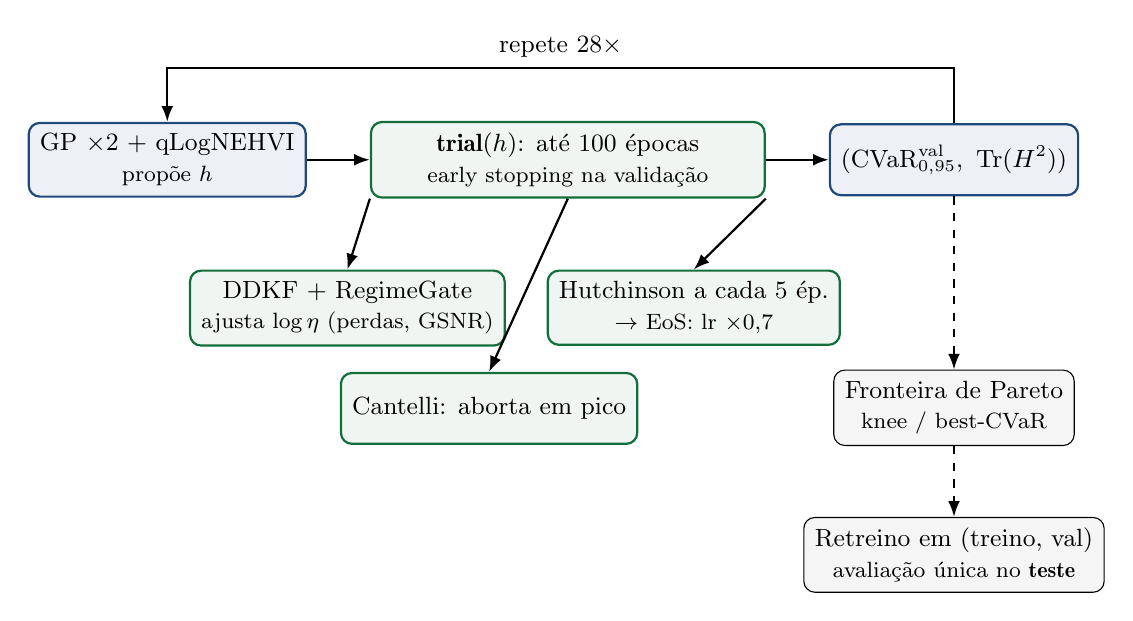
\begin{tikzpicture}[node distance=9mm and 8mm,
  box/.style={draw,rounded corners,align=center,minimum height=9mm,inner sep=4pt,fill=white,font=\small},
  macro/.style={box,fill=tune3blue!8,draw=tune3blue,thick},
  micro/.style={box,fill=okgreen!7,draw=okgreen,thick},
  arr/.style={-{Latex[length=2mm]},thick}]
\node[macro] (gp) {GP $\times2$ + qLogNEHVI\\ \footnotesize propõe $h$};
\node[micro,right=of gp,minimum width=50mm] (trial) {\textbf{trial}$(h)$: até 100 épocas\\ \footnotesize early stopping na validação};
\node[macro,right=of trial] (out) {$(\CVaR_{0{,}95}^{\text{val}},\ \Tr(H^2))$};
\node[micro,below=of trial,xshift=-28mm] (ddkf) {DDKF + RegimeGate\\ \footnotesize ajusta $\log\eta$ (perdas, GSNR)};
\node[micro,below=of trial,xshift=16mm] (eos) {Hutchinson a cada 5 ép.\\ \footnotesize $\to$ EoS: lr $\times0{,}7$};
\node[micro,below=of trial,yshift=-13mm,xshift=-10mm] (cant) {Cantelli: aborta em pico};
\node[box,below=of out,yshift=-13mm,fill=gray!8] (pareto) {Fronteira de Pareto\\ \footnotesize knee / best-CVaR};
\node[box,below=of pareto,fill=gray!8] (final) {Retreino em (treino, val)\\ \footnotesize avaliação única no \textbf{teste}};
\draw[arr] (gp) -- (trial);
\draw[arr] (trial) -- (out);
\draw[arr] (out.north) -- ++(0,7mm) -| node[pos=0.25,above,font=\small]{repete $28\times$} (gp.north);
\draw[arr] (trial.south west) -- (ddkf.north);
\draw[arr] (trial.south east) -- (eos.north);
\draw[arr] (trial.south) -- (cant.north);
\draw[arr,dashed] (out) -- (pareto);
\draw[arr,dashed] (pareto) -- (final);
\end{tikzpicture}
\caption{Visão geral do Tune3. À esquerda, o nível MACRO propõe hiperparâmetros e recebe dois objetivos por treinamento. Dentro de cada treinamento (nível MICRO), o DDKF ajusta a taxa de aprendizado a partir de perdas e GSNR; a curvatura alimenta o objetivo e o detector de EoS; o Cantelli aborta divergências. A avaliação final retreina a configuração escolhida usando \emph{apenas} treino e validação e toca no teste uma única vez.}
\end{figure}

\begin{algorithm}[H]
\caption{Um trial do Tune3 (\code{tune3/integration/trial.py})}
\KwIn{$h=(\eta_0,\lambda_{wd},p_{\text{drop}},\text{largura},\text{profundidade})$; treino $D_{tr}$; validação $D_{val}$}
inicializar MLP($h$), SGD($\eta_0$, momento $0{,}9$, $\lambda_{wd}$), DDKF($x_0=\log\eta_0$), RegimeGate, Cantelli, EoS, Hutchinson($M=5$)\;
\For{época $t=0,1,\dots,99$}{
  treinar uma época em $D_{tr}$ (lotes de 4096); guardar os gradientes dos 4 primeiros lotes\;
  $L^{tr}_t\leftarrow$ perda média de treino; \textbf{se} não finita: abortar\;
  $L^{val}_t$, perdas por amostra $\ell^{val}_t\leftarrow$ avaliar $D_{val}$ em \code{eval()}\;
  \If{$t \bmod 5=0$ \textbf{ou} última época}{
    $c_t\leftarrow\widehat{\Tr}(H^2)$ num lote de treino, em \code{eval()}; \quad $\text{eos}\leftarrow$ EoS.update($c_t$)\;
  }
  $z_t\leftarrow(L^{tr}_t, L^{val}_t, \log\GSNR_t)$; DDKF.update($z_t$); $R^2\leftarrow$ razão de informação; $\phi\leftarrow$ gating$(R^2)\in\{0,1\}$\;
  $\log\eta\leftarrow(1-\phi)\log\eta_{\text{atual}}+\phi\,\hat x_t$; \quad \textbf{se} eos: $\eta\leftarrow0{,}7\,\eta$\;
  \textbf{se} Cantelli.should\_abort($L^{val}_t$): abortar\;
  \textbf{se} $L^{val}_t$ melhorou ($>10^{-4}$): guardar $(\ell^{val}_t, c_t)$ como melhor época; zerar paciência; \textbf{senão} paciência$++$; \textbf{se} paciência $\ge10$: parar\;
}
\KwOut{$\CVaR_{0{,}95}(\ell^{val}_{\text{melhor}})$, $c_{\text{melhor}}$, telemetria (regimes, épocas com DDKF ativo, disparos do EoS)}
\end{algorithm}

\paragraph{Avaliação final e a separação treino/validação/teste.} Para cada método (Tune3 e comparadores), a configuração escolhida é \emph{retreinada} com um trial simples (sem DDKF) em (treino, validação): a melhor época é escolhida pela validação, o estado dessa época é restaurado e só então o modelo é avaliado no teste, uma única vez. O CVaR de teste dessa avaliação é a métrica primária. Isso implica algo que precisa ficar claro: \emph{o DDKF influencia a escolha dos hiperparâmetros, não o modelo final implantado}.

\begin{alerta}[O que estava errado antes]
Até setembro de 2026, o retreino final recebia o conjunto de \emph{teste} no lugar da validação: a melhor época era escolhida olhando o teste. Pela regra do próprio projeto, isso desqualifica os números anteriores de H1, H2 e H3, que precisam ser regerados com o pipeline corrigido. Um teste automatizado (\code{test\_A1}) agora garante que trocar o conjunto de teste não altera a época escolhida nem o CVaR de validação.
\end{alerta}

% =====================================================================
\section{Comparadores e desenho experimental}\label{sec:experimental}

\subsection{Dados e cenários}
DREBIN-215: $15\,036$ aplicativos Android, $215$ atributos binários de análise estática (permissões, \emph{intents}, chamadas de API), $\approx37\%$ malware. Divisão estratificada $80/20$ para teste e, do restante, $80/20$ para validação; a semente controla a divisão. Três cenários:
\begin{itemize}
\item \textbf{H1 --- in-distribution}: divisão aleatória estratificada;
\item \textbf{H2 --- desbalanceamento}: o malware do \emph{treino} é subamostrado para $5\%$, $2\%$ e $1\%$; validação e teste mantêm a composição natural;
\item \textbf{H3 --- zero-day por cluster}: o malware é agrupado por $k$-means em $5$ clusters no espaço de atributos; treina-se em $4$ e testa-se no cluster retido (proxy conservador de ``família nunca vista'', já que o DREBIN-215 não tem rótulos de família).
\end{itemize}

\subsection{Os oito métodos}
Todos recebem os mesmos dados, o mesmo espaço de busca (\code{log\_lr}$\in[-5,-2]$, \code{log\_wd}$\in[-6,-2]$, dropout $\in[0,0{,}5]$, largura $\in[32,256]$, profundidade $\in[1,4]$) e, exceto ASHA, o mesmo orçamento de $28$ treinamentos.

\begin{center}\small
\begin{tabular}{@{}llp{7.6cm}@{}}
\toprule
Método & Papel & O que isola \\ \midrule
\code{tune3\_bestcvar} & \textbf{primário} & ponto da fronteira com menor CVaR \\
\code{tune3} (knee) & alternativo & a configuração ``mais plana'' razoável --- se a geometria importa, deveria ganhar \\
\code{bo\_mono\_cvar} (B4) & E1 & mesma BO, mesmo trial interno, \emph{só} CVaR como objetivo: separa ``geometria'' de ``BO explora bem'' \\
\code{tune3\_placebo\_bestcvar} & E1 & 2\textsuperscript{o} objetivo $=$ ruído $\mathcal N(0,1)$: se empata com o Tune3, o ganho é da exploração bi-objetivo \\
\code{tune3\_noddkf\_bestcvar} & E2 & DDKF desligado (lr fixo): isola o nível MICRO \\
\code{random\_search} & baseline & controle ingênuo \\
\code{asha} & baseline & \emph{successive halving} (HPO moderno, orçamento em épocas) \\
\code{sam} & baseline & planura no espaço dos \emph{pesos} (SAM, $\rho=0{,}05$): o contraste direto com planura via hiperparâmetros \\
\bottomrule
\end{tabular}
\end{center}

\subsection{Protocolo estatístico (pré-registrado)}
Comparações pareadas por semente (mesmos splits para todos os métodos); Wilcoxon signed-rank bilateral; correção de Holm sobre a família de comparações; tamanho de efeito $d_z$ de Cohen (pareado) com intervalo de confiança bootstrap BCa (10\,000 reamostras); \textbf{vitória pré-registrada} $\Leftrightarrow$ $p_{\text{Holm}}<0{,}05$ \emph{e} $|d_z|\ge0{,}30$ \emph{e} direção favorável. Em H3, a unidade estatística é a semente (média sobre os 5 folds); a análise agrupando folds$\times$sementes é reportada apenas como exploratória, porque sementes do mesmo fold compartilham o conjunto de teste.

Uma nota sobre poder: o Wilcoxon bilateral com $n$ pares tem $p$ mínimo $2/2^n$; com $n<6$ é \emph{impossível} atingir $p<0{,}05$. Pilotos de 3 sementes validam o pipeline, não produzem significância. O protocolo usa 20 sementes (10 em H3), com ampliação única para 40 pré-declarada para casos inconclusivos.

% =====================================================================
\section{Estado da evidência e a tensão científica}\label{sec:evidencia}

\subsection{O que foi observado (com o pipeline anterior)}
\begin{center}\small
\begin{tabular}{@{}llp{8.2cm}@{}}
\toprule
Hipótese & Cenário & Resultado \\ \midrule
H1 & in-distribution & sem vantagem significativa do Tune3 \\
H2 & 5\% / 2\% / 1\% & direcional a favor de best-CVaR, sem significância ($d_z=0{,}04$--$0{,}20$) \\
H3 & zero-day & best-CVaR $\succ$ RS, ASHA e SAM, $p_{\text{Holm}}<0{,}001$; $|d_z|=0{,}46$ (RS/SAM) e $0{,}88$ (ASHA) \\
\bottomrule
\end{tabular}
\end{center}
\begin{alerta}[Validade]
Esses números foram produzidos com a avaliação final que escolhia a época no conjunto de teste (Seção~\ref{sec:algoritmo}). Eles orientam expectativas, mas \textbf{não podem ser reportados}. A reexecução com o pipeline corrigido é o primeiro item do protocolo pré-registrado.
\end{alerta}

\subsection{As três rachaduras na explicação geométrica}
Mesmo tomando H3 pelo valor de face, a explicação ``o Tune3 ganha \emph{porque} encontra mínimos planos'' tem três problemas:
\begin{enumerate}
\item \textbf{Correlação fraca, no cenário errado.} A correlação entre CVaR e curvatura medida foi $r=+0{,}26$ ($n=60$), e foi medida em H1 --- exatamente onde a teoria \emph{não} prevê vantagem. Em H3 ela nunca foi medida.
\item \textbf{A anomalia do knee.} O ponto \emph{mais plano} da fronteira (knee) tem CVaR consistentemente \emph{pior} que o best-CVaR. Se planura causasse baixo risco de cauda, o knee deveria ganhar. Ele perde.
\item \textbf{O comparador decisivo nunca rodou.} Sem B4 (BO mono-objetivo só em CVaR), não se distingue ``o mecanismo geométrico funciona'' de ``otimização bayesiana explora melhor o espaço que RS/ASHA''.
\end{enumerate}

\subsection{$H_G$ contra $H_M$}
\begin{center}
\begin{tabular}{@{}lp{10.5cm}@{}}
\toprule
$H_G$ (geométrica) & baixa curvatura \emph{causa} baixo CVaR e robustez a variantes não vistas \\
$H_M$ (exploração) & o ganho vem da exploração multi-objetivo do espaço de hiperparâmetros; a curvatura é um segundo objetivo qualquer \\
\bottomrule
\end{tabular}
\end{center}
A evidência disponível é \emph{mais consistente com $H_M$}. Isso não é uma derrota: é a pergunta que a Linha 1 existe para responder.

\subsection{Linha 1: E0, E1, E2 e a árvore de decisão}\label{sec:linha1}
\begin{itemize}
\item \textbf{E0} --- correlação \emph{parcial} entre CVaR e $\log\Tr(H^2)$ dentro dos folds de H3, controlando $\log\eta$ e $\log\lambda_{wd}$ (\code{scripts/analyze\_e0.py}). $H_G$ prevê correlação parcial positiva com IC excluindo zero. Só é válida sobre resultados gerados pelo pipeline corrigido.
\item \textbf{E1} --- B4 e placebo, mesmo orçamento. $H_G$ prevê que o Tune3 vence \emph{ambos}; $H_M$ prevê empate com o placebo e/ou derrota para B4.
\item \textbf{E2} --- DDKF ligado vs.\ desligado, com a telemetria de engajamento. Se o DDKF quase nunca sai do regime A, o nível MICRO é declarado inerte, seja qual for o CVaR.
\end{itemize}
\begin{center}\small
\begin{tabular}{@{}llp{7cm}@{}}
\toprule
Cenário & Condição & Consequência \\ \midrule
C1 & Tune3 vence B4 e placebo; E0 positiva & $H_G$ sobrevive $\to$ H4 (robustez adversarial) \\
C2 & placebo empata com Tune3 & reposicionar a tese em torno da exploração multi-objetivo \\
C3 & empate geral & artigo de metodologia de avaliação \\
C4 & B4 vence Tune3 & parada obrigatória e reunião de coordenação \\
\bottomrule
\end{tabular}
\end{center}
Nenhum dos quatro é fracasso; cada um leva a um artigo diferente. O que seria fracasso é escrever qualquer deles antes de os dados decidirem.

% =====================================================================
\section{Literatura: o que cada artigo sustenta --- e o que não sustenta}\label{sec:literatura}

A tabela abaixo reproduz a leitura \emph{corrigida} do corpus do projeto (auditoria de 07/09/2026), após a descoberta de que uma versão anterior do material de apoio continha uma referência inexistente e quatro atribuições indevidas.

\begin{center}\small
\begin{tabular}{@{}p{3.1cm}p{5.4cm}p{6.3cm}@{}}
\toprule
Referência & Sustenta & Não sustenta \\ \midrule
Sagun, Bottou, LeCun (2017)~\cite{sagun2017} & espectro da Hessiana degenerado: bulk em zero + poucos outliers & que os outliers dominem o traço em \emph{qualquer} arquitetura (verificar no MLP do DREBIN: razão $\lambda_{\max}^2/\Tr(H^2)$) \\
Yao et al.\ (2018)~\cite{yao2018} & correlação \emph{empírica} entre espectro de $H_\theta$ e robustez, mediada pelo \emph{batch size} & relação matemática $\lambda_{\max}\leftrightarrow$ sensibilidade; o teorema do artigo é sobre $H_x$ (entrada), não $H_\theta$; com $B$ fixo, o desenho não transfere ao Tune3 \\
Hochreiter, Schmidhuber (1997)~\cite{hochreiter1997} & mínimos planos têm menor complexidade descritiva (MDL) & aplicabilidade direta a redes ReLU modernas (ver Dinh et al.~\cite{dinh2017}) \\
Foret et al.\ (2021)~\cite{foret2021} & SAM: min-max sobre $\theta$ melhora generalização em visão & que atuar em $h$ produza o mesmo efeito --- isso \emph{é} a hipótese do Tune3 \\
Zhang et al.\ (\textbf{2023}, ICCV)~\cite{zhang2023} --- método \textbf{FAD} & planura ajuda em generalização de domínio (\emph{out-of-distribution}) & transferência automática para zero-day em malware \\
Cohen et al.\ (2021)~\cite{cohen2021} & \emph{progressive sharpening} e EoS em GD \textbf{full-batch} & comportamento sob SGD com minibatches (o caso do Tune3) \\
Ly, Gong (2025)~\cite{ly2025} & paisagem multifractal; GD encontra mínimos planos \emph{automaticamente} & que otimizadores convencionais falhem por causa da multifractalidade \\
Tsipras et al.\ (2019)~\cite{tsipras2019} & trade-off robustez $\times$ acurácia (útil para a fronteira de Pareto) & --- (não está no corpus de PDFs; avaliado por conhecimento do artigo) \\
Hutchinson (1990)~\cite{hutchinson1990}; PyHessian~\cite{yao2020} & estimador de traço; ferramentas de espectro & --- \\
\bottomrule
\end{tabular}
\end{center}

\begin{alerta}[Referência inexistente]
``Gholami et al.\ (2019), \emph{Anatomy of Hessian}'' não existe. O PDF homônimo que circulou no corpus é de Sonbolestan e \emph{Ali} Gholami (geofísica, inversão sísmica) e não tem relação com redes neurais. As referências corretas para o cálculo espectral são Hutchinson (1990) e PyHessian~\cite{yao2020}.
\end{alerta}

\paragraph{Terminologia.} Usar \emph{geométrico} para propriedades quantificáveis via curvatura (Hessiana, autovalores, norma de Frobenius); reservar \emph{topológico} para invariantes sob deformação contínua. ``Blindagem topológica'' deve ser lida como ``blindagem geométrica'' --- e, enquanto $H_G$ não for confirmada, como \emph{hipótese} de blindagem.

% =====================================================================
\section{Glossário de símbolos}
\begin{center}\small
\begin{tabular}{@{}lp{11.5cm}@{}}
\toprule
$\theta\in\R^W$ & pesos da rede \\
$h\in\mathcal H\subset\R^5$ & hiperparâmetros: $\log_{10}\eta$, $\log_{10}\lambda_{wd}$, dropout, largura, profundidade \\
$L$, $\ell$ & perda média; perdas por amostra \\
$\CVaR_\gamma$, $\gamma=0{,}95$ & média dos $5\%$ piores casos \\
$H_\theta$, $\Tr(H^2)=\norm{H}_F^2$ & Hessiana da perda nos pesos; curvatura agregada \\
$v_i$, $M$ & sondas de Rademacher; número de sondas ($5$ no treino) \\
$\GSNR$ & $\norm{\bar g}^2/\Tr(\Sigma)$, razão sinal-ruído do gradiente \\
$x_t=\log\eta_t$, $\rho$, $\sigma_\eta$ & estado do DDKF; $\rho=0{,}95$, $\sigma_\eta=0{,}05$ \\
$z_t$ & observação do DDKF: $(L^{tr},L^{val},\log\GSNR)$ \\
$P_{xz},P_{zz},K,u_t$ & covariâncias empíricas, ganho, correção escalar \\
$R^2=S_u/S_\infty$ & razão de informação; regimes A/B/C em $0{,}10$ e $0{,}50$ \\
$k_\gamma=\sqrt{\gamma/(1-\gamma)}$ & constante de Cantelli ($\approx4{,}36$) \\
$d_z$, $p_{\text{Holm}}$ & tamanho de efeito pareado; $p$ corrigido \\
\bottomrule
\end{tabular}
\end{center}

% =====================================================================
\appendix
\section{Mapa teoria \texorpdfstring{$\leftrightarrow$}{<->} código}\label{ap:mapa}
\begin{center}\footnotesize
\begin{tabular}{@{}p{3.3cm}p{6.3cm}p{5.6cm}@{}}
\toprule
Conceito & Arquivo & Classe / função \\ \midrule
CVaR (Eq.~\ref{eq:ru}) & \code{tune3/core/objectives.py} & \code{cvar}, \code{cvar\_rockafellar} \\
Hutchinson (Eq.~\ref{eq:hutch}) & \code{tune3/curvature/hutchinson.py} & \code{HutchinsonEstimator.estimate} \\
GSNR & \code{tune3/curvature/gsnr.py} & \code{GSNREstimator.from\_gradients} \\
DDKF (Eq.~\ref{eq:ar1}, \ref{eq:obs}) & \code{tune3/micro/ddkf\_controller.py} & \code{DDKFController.update}, \code{information\_ratio} \\
Regimes A/B/C & \code{tune3/micro/regime\_gating.py} & \code{RegimeGate} \\
Cantelli & \code{tune3/safety/cantelli.py} & \code{CantelliGuard.should\_abort} \\
EoS & \code{tune3/safety/eos\_detector.py} & \code{EoSDetector.update} \\
Trial (Alg.~1) & \code{tune3/integration/trial.py} & \code{run\_trial} \\
MACRO (GP + EHVI) & \code{tune3/macro/bo\_loop.py} & \code{Tune3MacroLoop} \\
Placebo (E1) & \code{tune3/integration/runner.py} & \code{Tune3RunConfig.objective2} \\
B4 (E1) & \code{tune3/baselines/bo\_mono.py} & \code{MonoObjectiveBO} \\
RS, ASHA, SAM & \code{tune3/baselines/hpo.py}, \code{sam.py} & --- \\
Avaliação final & \code{tune3/baselines/plain\_trial.py} & \code{plain\_trial(..., test\_data=)} \\
Protocolos H1 / S1 / S2 & \code{tune3/experiments/protocol.py}, \code{tune3/experiments/security\_protocol.py} & \code{run\_protocol}, \code{run\_security\_protocol} \\
Estatística & \code{tune3/experiments/stats.py} & \code{compare\_paired}, \code{bootstrap\_ci} \\
E0 & \code{scripts/analyze\_e0.py} & --- \\
Validação teoria$\times$código & \code{scripts/validate\_theory.py} & V1--V9 (13 itens) \\
\bottomrule
\end{tabular}
\end{center}

\paragraph{Procedência das referências.} As entradas marcadas com $\star$ foram conferidas, em setembro de 2026, contra o PDF do próprio artigo no acervo do projeto (ou, quando indicado, contra a bibliografia do documento de projeto que acompanha o acervo). As demais foram transcritas de documentos internos anteriores e \textbf{ainda não foram conferidas em fonte primária} --- trate-as como indicação de leitura, não como citação verificada.

\begin{thebibliography}{99}\small
\bibitem{rockafellar2000} R.\,T.\ Rockafellar, S.\ Uryasev. Optimization of conditional value-at-risk. \emph{Journal of Risk} 2(3):21--41, 2000.
\bibitem{hutchinson1990} $\star$ M.\,F.\ Hutchinson. A stochastic estimator of the trace of the influence matrix for Laplacian smoothing splines. \emph{Communications in Statistics --- Simulation and Computation} 19(2):433--450, 1990.
\bibitem{yao2020} Z.\ Yao, A.\ Gholami, K.\ Keutzer, M.\,W.\ Mahoney. PyHessian: Neural networks through the lens of the Hessian. \emph{IEEE Int.\ Conf.\ on Big Data}, 2020 (arXiv:1912.07145).
\bibitem{liu2020} J.\ Liu et al. Understanding why neural networks generalize well through GSNR of parameters. \emph{ICLR}, 2020.
\bibitem{sagun2017} $\star$ L.\ Sagun, L.\ Bottou, Y.\ LeCun. Eigenvalues of the Hessian in deep learning: singularity and beyond. arXiv:1611.07476v2, 5 out.\ 2017.
\bibitem{yao2018} $\star$ Z.\ Yao, A.\ Gholami, Q.\ Lei, K.\ Keutzer, M.\,W.\ Mahoney. Hessian-based analysis of large batch training and robustness to adversaries. \emph{NeurIPS}, 2018.
\bibitem{hochreiter1997} $\star$ S.\ Hochreiter, J.\ Schmidhuber. Flat minima. \emph{Neural Computation} 9(1):1--42, 1997.
\bibitem{dinh2017} L.\ Dinh, R.\ Pascanu, S.\ Bengio, Y.\ Bengio. Sharp minima can generalize for deep nets. \emph{ICML}, 2017.
\bibitem{foret2021} $\star$ P.\ Foret, A.\ Kleiner, H.\ Mobahi, B.\ Neyshabur. Sharpness-aware minimization for efficiently improving generalization. \emph{ICLR}, 2021.
\bibitem{zhang2023} $\star$ X.\ Zhang, R.\ Xu, H.\ Yu, Y.\ Dong, P.\ Tian, P.\ Cui. Flatness-aware minimization for domain generalization. \emph{ICCV}, pp.\ 5189--5202, 2023. (O método proposto chama-se \textbf{FAD}, \emph{Flatness-Aware minimization for Domain generalization}.)
\bibitem{cohen2021} $\star$ J.\,M.\ Cohen, S.\ Kaur, Y.\ Li, J.\,Z.\ Kolter, A.\ Talwalkar. Gradient descent on neural networks typically occurs at the edge of stability. \emph{ICLR}, 2021.
\bibitem{ly2025} $\star$ A.\ Ly, P.\ Gong. Optimization on multifractal loss landscapes explains a diverse range of geometrical and dynamical properties of deep learning. \emph{Nature Communications} 16:3252, 2025.
\bibitem{tsipras2019} D.\ Tsipras, S.\ Santurkar, L.\ Engstrom, A.\ Turner, A.\ Madry. Robustness may be at odds with accuracy. \emph{ICLR}, 2019.
\bibitem{daulton2021} S.\ Daulton, M.\ Balandat, E.\ Bakshy. Parallel Bayesian optimization of multiple noisy objectives with expected hypervolume improvement. \emph{NeurIPS}, 2021.
\bibitem{ament2023} S.\ Ament, S.\ Daulton, D.\ Eriksson, M.\ Balandat, E.\ Bakshy. Unexpected improvements to expected improvement for Bayesian optimization. \emph{NeurIPS}, 2023.
\bibitem{li2020} L.\ Li et al. A system for massively parallel hyperparameter tuning (ASHA). \emph{MLSys}, 2020.
\bibitem{arp2014} D.\ Arp, M.\ Spreitzenbarth, M.\ Hübner, H.\ Gascon, K.\ Rieck. DREBIN: Effective and explainable detection of Android malware in your pocket. \emph{NDSS}, 2014.
\bibitem{oliveira2025} de Oliveira, Diniz, Kreutz, Schmidt, Mansilha. Tune3: Otimização multiestágio de hiperparâmetros com redução de custo e maior estabilidade em modelos de detecção de malware Android. \emph{Anais do 9º WRSeg}, 2025 (menção honrosa).
\end{thebibliography}

\end{document}
